%Thus far in this work a solution to simplify and automate design the process of all digital PLL loop filter designs comprised of (1) an automated loop filter optimization and design engine, and (2) a discrete-event, time domain PLL simulator to evaluate the designed filters with full time-discretization and quantization nonlinearity effects. I
In this discussion, the performance of the implemented design will first be analyzed via comparison to a theoretically calculated jitter limit, and then will be compared to current state of art. Small area and low power PLLs are considered for reference. Later, identified areas of improvement within the presented design are discussed.

\subsection{Performance Limit for Ring Oscillator BBPD PLLs with PI-controllers}\label{sec:fomjit_limit}
	In the case of a perfect ring oscillator PLL, all components would be noiseless and consume minimal energy possible. For an ADPLL, the consideration of power can be divided between logic and the oscillator. In the case of logic, the theoretical energy limit for switching of a logical level of a gate equates to $E_s = \ln(2) k_B T$, \cite{Lundstrom2006}. With a reference frequency of $f_{ref}$, and $N$ digital nodes, the minimum possible power expenditure from digital components of PLL is in equation \ref{eq:min_sw_energy}. This assumes the worst case scenario where all gates switch every cycle.
	\begin{equation}\label{eq:min_sw_energy}
		P_{min,digital} = Nf_{ref}\ln(2) k_B T
	\end{equation}
	At 300 K, the design considered in this work having complexity of logic N $\approx$ 1000, and $f_{ref}$ = 16 MHz, yields a \textit{theoretical} consumption of 66 pW, practically zero. Infact, it is found \textit{theoretically} that the one can operate 242 thousand gates at 1 GHz and consume only 1 $\mu$W of power. Following these findings, and considering total PLL operating power on the regime of 100 $\mu$W, it has been assumed here that the theoretical power limit for digital components of an ADPLL is practically zero. In the case of a ring oscillator, however, power may not be scaled to zero as with logic. This is due to the fundamental relationship between oscillator power and phase noise, as discussed in section \ref{sec:ro_pn_limit}. Therefore, it is now asserted that an optimal (AD)PLL will expend all of its power in its oscillator. Analyzing the case presented in this work of a BBPD and PI-controller based PLL, it was determined that the expected value of total phase noise is in equation \ref{eq:optimal_pn_pow}. Using the theoretical limit of ring oscillator phase noise in equation \ref{eq:ro_pn}, the result of equation \ref{eq:min_pibbpdpll_pn} provides the minimum achievable PI-controller BBPD PLL phase noise.
	\begin{equation}\label{eq:min_pibbpdpll_pn}
		\sigma_{\Phi_{n,opt}}^2 = 74.79376\cdot \frac{\mathcal{L}_{min}(f)f^2}{f_{ref}} = 74.79376\cdot  \frac{7.33 k_B T f_{osc}^2}{f_{ref}P_{DC}}
	\end{equation}

	 This result can be converted into RMS jitter, with $\sigma_{\Phi_{n}} = 2\pi f_{osc}\sigma_{j_t}$, yielding equation \ref{eq:min_pibbpdpll_jit}.
	\begin{equation}\label{eq:min_pibbpdpll_jit}
		\sigma_{j_t}^2 = 74.79376\cdot  \frac{7.33 k_B T}{(2\pi)^2f_{ref}P_{DC}}
	\end{equation}


	  Using the FOM$_{jitter}$ expression in equation \ref{eq:ro_fom_limit}, it is seen that the theoretical limit for PLL FOM of the PI-controller BBPD-PLL is in equation \ref{eq:ro_fom_jit_limit}. Noting the dependence on reference frequency, with $f_{ref}$ = 16 MHz at 300 K, this is -234.4 dB. Equation \ref{eq:ro_fom_jit_fom_pn} provides the general expression for FOM$_{jitter}$ limit provided an oscillator FOM$_{pn}$ value. It should be noted that the only way to improve jitter FOM in the proposed architecture is to reduce temperature, increase frequency, or improve oscillator FOM (that is, use a resonant oscillator, such as an LC oscillator).
	\begin{equation}\label{eq:ro_fom_jit_limit}
		\textnormal{FOM}_{\textnormal{jitter,min}} = 10\log_{10}\left(\frac{\sigma_{t_j}^2}{(\textnormal{1 s})^2}\cdot\frac{P_{DC}}{\textnormal{1 mW}}\right) =  10\log_{10}\left( 74.79376\cdot  \frac{7.33\times 10^3 k_B T}{(2\pi)^2f_{ref}} \right)
	\end{equation}
	\begin{equation}\label{eq:ro_fom_jit_fom_pn}
		\textnormal{FOM}_{\textnormal{jitter,min}} = \textnormal{FOM}_{pn} + 10\log_{10}\left(\frac{74.79376}{(2\pi)^2 f_{ref}} \right)
	\end{equation}

\subsection{State of Art}
% \hl{RM lock time part}

In order to form a comparison to the current state of art for ultra low power PLLs, a wide search of literature was undertaken, and data from relevant PLL designs were collected into table \ref{tab:state_of_art}. Specific criteria for this search were power consumption below 1 mW, publication within 2 years of this work, similar oscillation frequency, and preference to ring oscillator designs implementing integer-N architectures. Filtering in this manner has resulted in a curated selection of 5 highly comparable designs to the one of this work.

Analyzing FOM$_{jitter}$, this work is on the lower end of being state of art, achieving -225 dB, where the observed range was [-236.8,-226.1] dB for the selected works. Using the theoretical limit for FOM$_{jitter}$ in this topology derived in \ref{sec:fomjit_limit}, the best achievable value of FOM$_{jitter}$ possible with this work using a ring oscillator is -234.4 dB (at 300K and $f_{ref}$ = 16 MHz). Adding a penalty for consuming power in non-oscillator components (5 $\mu$W of the 95 $\mu$W power consumption) results in a 0.5 dB reduction from the optimal jitter FOM. Furthermore, the obtained oscillator phase noise FOM of -158.9 dB, being 6.3 dB worse than the theoretically obtainable -165.2 dB, adds an additional penalty of 6.3 dB. Thus the realistic best case result in this design including the penalties is therefore -227.6 dB, which explains the positioning of this work on the low end of FOM$_{jitter}$ for comparable designs. In equation \ref{eq:ro_fom_jit_fom_pn}, oscillator FOM is seen to be improved with increasing reference frequency. In this work, however, a higher reference frequency was not an option, as this design was constrained with a 32 MHz reference frequency, and this must be divided to 16 MHz to achieve an integer ratio to the target RF frequency of 2448 MHz. If it were possible to increase the reference frequency, for example to 200 MHz as in Xiang'20 \cite{Xiang2020}, the theoretical FOM$_{jitter}$ then is extended to -245.4 dB, or -238.6 dB penalized, bringing the FOM to be highly competitive with the other works. As a general statement, the FOM$_{jitter}$ of this work is necessarily limited by the design constraints imposed on the design.

This work comes out ahead of existing designs in terms of total power consumption, where sub-100$\mu$W is achieved, a feat that was not paralleled by any of the surveyed works. In the application area of this work to duty cycled wake up receivers, fast locking and ultra low power consumption are of primary interest in terms of PLL performance. While the other surveyed designs obtain better phase noise performance than this work with simultaneously higher power consumption, this design has been optimized to have sufficiently good phase noise for the target application while preferring reduction in power over improving phase noise. Furthermore, the architectural choices of this work have been implemented to favor fast locking, on the order of 664 ns, compared to the other design which make no mention of locking performance, require long lock times, in upwards of 120$\mu$s (1200 cycles at 10 MHz) in the case of Liu'19, or have prohibitively high power with 682 $\mu$W in Xiang'20 to obtain a 200 ns locktime. It is therefore ascertained that this work meets the needs of the end use for wake up receivers better than the surveyed literature, providing merit to the design beyond the pure phase noise performance results.

In terms of oscillator performance, this design shows improvements again in power versus others, utilizing only 90$\mu$W. The next closest work in oscillator power is that by Liu'19 \cite{Liu2019}. That design uses an LC VCO with a SSB phase noise of -107 dBc/Hz at 1 MHz for a 2.46 GHz frequency, yielding an oscillator FOM of -184.5 dB. The oscillator is only a single stage differential LC oscillator, consuming 107 $\mu$W. Practically, the PLL of this work is required to generate quadrature signals, so the non-quadrature 107 $\mu$W of that work should be doubled, i.e. to 214 $\mu$W, to estimate power consumption for quadrature phase generation. A new oscillator FOM of -181.5 is achieved, which is 22.6 dB improved over the -158.9 dB achieved in this work. It is not expected that the remaining works are substantially better than this work in terms of phase noise, due to them being ring oscillator based, coupled with the theoretical limit of -165.2 dB for FOM phase noise at 300 K. Based purely on oscillator phase noise values, and the prediction for PI-controller BBPD-PLL FOM$_{jitter}$ in equation \ref{eq:ro_fom_jit_fom_pn}, the LC-based PLL should be expected to achieve \textit{at least} 22.6 dB better FOM$_{jitter}$ than this work. However, this is not completely observed, Liu only reports -236.8 dB FOM$_{jitter}$, an improvement of 11.8 dB over this work. This discrepancy is probably due to the FLL architecture used in that work. It appears that the oscillator core from Liu's work, coupled with the PLL topology of this work, would yield a FOM$_{jitter}$ of -248.0 dB, substantially better than that demonstrated in either work. It is a question, perhaps for future work, to determine if an LC oscillator core can be used satisfactorily with the topology of this work for the needs of wake up receivers. Issues cropping up related to the LC oscillator may prove challenging due to non-instantaneous startup, and inability to reset oscillator phase to be clock synchronous instantly, which may overall lead to locking instability with the BBPD-PLL. 

In regards to implementation area, this work is highly competitive to current state of art design, only beat in area by 1\% by a fractional-N PLL built in 5nm technology by Liu'20 \cite{Liu2020}. This should be expected due to substantially smaller devices and metal pitch in 5nm versus the 22nm in this work. The LC based design by Liu'19 achieved an area 49x of this work, which was limited by integration area needed by the resonant LC circuit to have sufficiently high-Q. The analog designs also came close in area. The design implemented by Zhang'19 \cite{Zhang2019} in 40 nm technology came close with only 2.39x greater area than this work.

Concerning analog versus digital implementation, the two analog ring-oscillator PLL designs (Zhang'19 \cite{Zhang2019} and Xiang'20 \cite{Xiang2020}) are comparable in terms of FOM, however, power is not seen to scale as low as this work. Both designs also employ higher reference frequencies than here, being 100 MHz \cite{Zhang2019} and 200 MHz \cite{Xiang2020}, which is expected to help reduce phase noise contribution from the oscillator significantly, as much higher loop bandwidth can be used, bringing down the in-band phase noise level. The analog designs discussed here are both phase-frequency detector (PFD) and charge pump (CP) based, which exhibit linear dynamics \cite{Razavi2020}, in comparison to the BBPD design of this work that is inherently nonlinear due to its detector characteristics. As seen in this work, BBPD designs can exhibit undesirable emergent behaviors, potentially leading to cyclostationary phase trajectories and increased phase noise contributions if not properly designed. This hazard can be mitigated with linearized designs, for example employing a PFD-CP architecture. It is expected, though, that analog implementations will introduce different non-idealities into the PLL, namely extra analog noise into the loop, which may negate any advantages. It is possible to implement a PFD-PLL with a digital CP loop filter to remove these noise sources, as Palaniappan'18 \cite{Palaniappan2018} does. In that work, a comparable FOM to this work of -226.1 dB was seen, albeit at a lower output frequency of circa 400 MHz. According to \cite{xu_abidi_2017}, the PFD-CP approach is not necessarily better, as in practice, equal performance in terms of total jitter is achievable with BBPD and charge pump designs \textit{if} properly optimized. Furthermore, implementation complexity is higher for a PFD, nominally requiring two D flip flops and an AND gate \cite{Razavi2020}, whereas a BBPD is as simple as a single D flip flop. Thus, when scaling for minimum power, lower power should be achievable with a BBPD as it is simpler. Overall, it does not appear that either analog implementation or CP-PFD designs pose any significant advantages to this work in the ultra low power regime when considering the design of a 100$\mu$W PLL. Rather, digital implementation is perhaps more favorable due to lower sensitivity to PVT variation.

% In terms of lock time, highly favorable performance was seen in the analog design of Xiang, with circa 0.2 $\mu$s. However, a high reference frequency of 200 MHz is used, or equivalently 20 reference cycles. 20 reference cycles in this work is 1.25 $\mu$s, so it is more comperable to this work. Inspecting the the best FOM result of the table ). This FLL approach does not appear viable for fast start of needs in WUR.
Two of the reviewed papers presented interesting comparison figures for (a) PLL jitter FOM versus power consumption, in figure \ref{fig:fom_v_pow}, and (b), jitter FOM versus implementation area, in figure \ref{fig:fom_v_area}. The works that the figures were published in are from 2019 and 2020 respectively. With the PLL of this work having a power consumption of sub-100 $\mu$W, a FOM$_{jitter}$ of -225 dB, and area of 0.00365 mm$^2$, it is seen that this design lands off the chart, beyond the suggested FOM trend line in power versus FOM, and lands in a comparable position with other recent design in terms of FOM versus area. Based on this comparison, it is concluded that this work is boundary pushing in terms of power consumption, and is also state of art in area of implementation.
\FloatBarrier\pagebreak

	\begin{figure}[htb!]
	    \centering
	    \begin{subfigure}{0.5\textwidth}
	        \centering
	        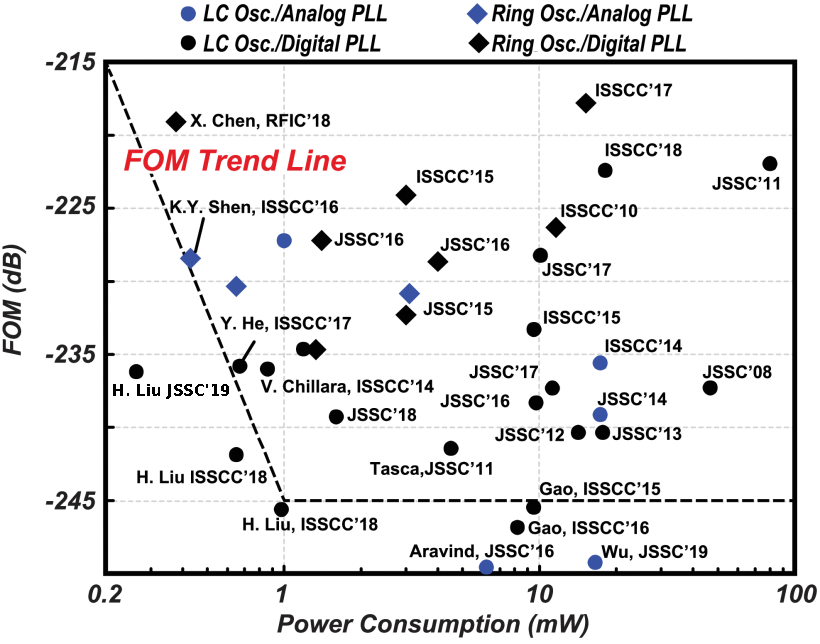
\includegraphics[width=1\textwidth, angle=0]{./figs/liu24-fom2}
	        \caption{ }
	        \label{fig:fom_v_pow}
	    \end{subfigure}%
	    \begin{subfigure}{0.5\textwidth}
	        \centering
	        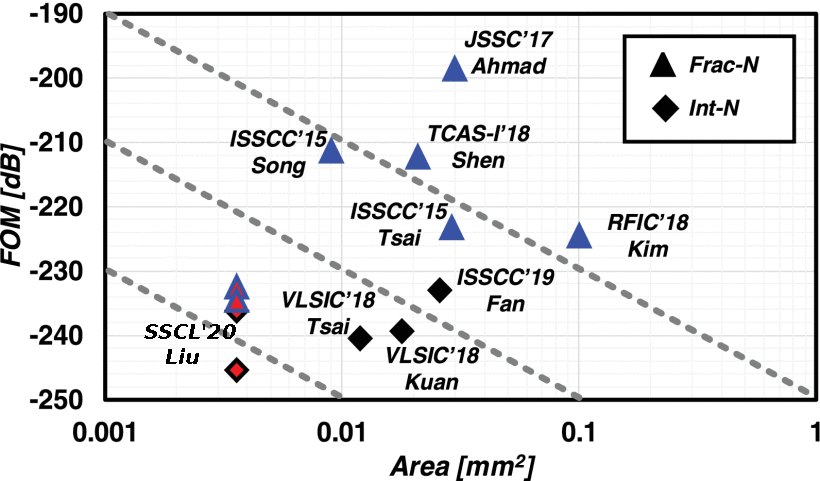
\includegraphics[width=1\textwidth, angle=0]{./figs/liu_5nm2}
	        \caption{ }
	        \label{fig:fom_v_area}
	    \end{subfigure}
	    \caption{\textbf{(a)} FOM$_{jitter}$ versus power modified from \cite{Liu2019} (JSSC 2019), \textbf{(b)} FOM$_{jitter}$ versus area modified from \cite{Liu2020} (SSCL 2020).}
	    \label{fig:fom_charts}
	\end{figure}


	% \FloatBarrier
	\begin{table}[h!]
		\centering
		\def\arraystretch{1.5}		
		\setlength\arrayrulewidth{0.75pt}
		\setlength{\tabcolsep}{0.5em} % for the horizontal padding
		\begin{tabular}{|>{\centering}m{0.2\textwidth}?>{\centering}m{0.1\textwidth}?>{\centering}m{0.11\textwidth}|>{\centering}m{0.1\textwidth}|>{\centering}m{0.1\textwidth}?>{\centering}m{0.11\textwidth}|>{\centering\arraybackslash}m{0.1\textwidth}|}
			\hline 
			\rule[-1ex]{0pt}{2.5ex} \cellcolor{gray!40}\textbf{Parameter} & \cellcolor{gray!40}\textbf{This Work} & \cellcolor{gray!40}\textbf{JSSC'19 Liu} \cite{Liu2019} & \cellcolor{gray!40}\textbf{{\footnotesize NORCHIP'18 Palaniappan} }\cite{Palaniappan2018} & \cellcolor{gray!40}\textbf{SSCL'20 Liu} \cite{Liu2020} & \cellcolor{gray!40}\textbf{2019 Zhang} \cite{Zhang2019} & \cellcolor{gray!40}\textbf{CICC'20 Xiang} \cite{Xiang2020} \\
			\hline 
			\rule[-1ex]{0pt}{2.5ex} \textbf{Analog/Digital} & Digital  & Digital  & Digital & Digital & Analog & Analog \\
			\hline 
			\rule[-1ex]{0pt}{2.5ex} \textbf{Int-N/Frac-N} & Int-N  & Frac-N  & Int-N & Int-N & Int-N & Int-N  \\
			\hline 
			\rule[-1ex]{0pt}{2.5ex} \textbf{Architecture} & BB-PLL\tablefootnote{BBPD PLL} & FLL + ODZ\tablefootnote{Out of deadzone detector}  & {Digital CP-PLL\tablefootnote{Charge Pump PLL}} & IL-PLL\tablefootnote{Injection-locked PLL} & CP-PLL & CP-PLL \\
			\hline 
			\rule[-1ex]{0pt}{2.5ex} \textbf{Process} & 22nm & 65nm & 40nm & 5nm & 40nm & 22nm \\
			\hline 
			\rule[-1ex]{0pt}{2.5ex} \textbf{Osc. Type} & RO & LC & RO & RO & RO  & RO \\
			\hline 
			\rule[-1ex]{0pt}{2.5ex} \textbf{Detector} & BBPD & ODZ & PFD\tablefootnote{Phase-frequency detector} & Sampling & PFD & PFD\\
			\hline
			\rule[-1ex]{0pt}{2.5ex} \textbf{Area [mm$^2$]} & 0.00365 & 0.25 & 0.0186 & 0.0036 & 0.00873 & 0.015 \\
			\hline 
			\rule[-1ex]{0pt}{2.5ex} \textbf{Power [$\mu$W]} & 95 & 265 & 270.5 & 440 & 170  & 682 \\
			\hline 		 
			\rule[-1ex]{0pt}{2.5ex} \textbf{f$_{ref}$ [MHz]} & 16 & 10 & - & 40 & 100 & 200 \\
			\hline 
			\rule[-1ex]{0pt}{2.5ex} \textbf{f$_{osc}$ [GHz]} & 0.816 & 2.1-3.1 & 330-470 & 1.0 & 1.6 & 3.2 \\
			\hline 
			\rule[-1ex]{0pt}{2.5ex} \textbf{Osc. Stages (N$_{stg}$)} & 6 & 1 & 8 & - & 3 & - \\
			\hline 
			\rule[-1ex]{0pt}{2.5ex} \textbf{f$_{osc}$ $\times$ N$_{stg}$} [GHz] & 4.896 & 2.1-3.1 & 2640-3760 & - & 4.8 & - \\
			\hline 	
			\rule[-1ex]{0pt}{2.5ex} \textbf{Osc. Power [$\mu$W]} & 90.4 & 107 & - & 398 & - & 225 \\
			\hline 		
			\rule[-1ex]{0pt}{2.5ex} \textbf{Jitter [ps$_{\textnormal{\textbf{RMS}}}$]} & 18.4  & 2.8 & 9.53 & 2.34 & 8.3 & 2.3 \\
			\hline 			
			\rule[-1ex]{0pt}{2.5ex} \textbf{$\textnormal{FOM}_{\textnormal{jitter}}$ [dB]} & -225.0  & -236.8 & -226.1 & -236.2 & -229.3 & -234.3 \\
			\hline 		
			\rule[-1ex]{0pt}{2.5ex} \textbf{Lock-time [$\mu$s]} & 0.664 & $\leq$ 120  & - & - & - & 0.2 \\
			\hline 			
		\end{tabular} 
		% \caption{Assigned specifications for branch line hybrid design.}
		% \label{asgn_specs}
		\caption{State of art comparison of PLLs.}
		\label{tab:state_of_art}
	\end{table}  



	% \begin{figure}[htb!]
	% 	\center\includegraphics[width=1.0\textwidth, angle=0]{figs/x.pdf}
	% 	\caption{Transient simulation of optimal design.}
	% 	\label{fig:des_ex_trans}
	% \end{figure}
	% \FloatBarrier

	% \begin{figure}[htb!]
	% 	\center\includegraphics[width=1.0\textwidth, angle=0]{figs/x.pdf}
	% 	\caption{Variation Simulation for KDCO.}
	% 	\label{fig:var_lock}
	% \end{figure}
	% \FloatBarrier

	% \begin{figure}[htb!]
	% 	\center\includegraphics[width=1.0\textwidth, angle=0]{figs/x.pdf}
	% 	\caption{Phase noise.}
	% 	\label{fig:Simulated phase noise.}
	% \end{figure}
	% \FloatBarrier

	% stability criteria - Jurys' stability criteria abs(a0) l.t. a2 for second order z-transfer \cite{xiu_li_meiners_padakanti_2004}
	% - Not phase margin based in optimization, can make stable by using stable choice of PI controller (two poles only) - poles should be in unit circle...
\FloatBarrier



\subsection{Radio System Performance}
	For the specified radio system in which this PLL has been designed to enable, a requirement of $\leq$ 20.56 ps RMS integrated jitter was defined to ensure satisfactory bit error rate performance. In this work, the implemented design meets this requirement, with an observed RMS jitter of 18.4 ps (see table \ref{tab:pll_pn_jit_vals}). Furthermore, the power requirement of $\leq$ 100 $\mu$W is obtained, with 95 $\mu$W of power consumption realized. Finally, the implemented PLL enables IQ sampling at 2.448 GHz through oversampling at the 1/3 subharmonic (816 MHz), satisfying the last major requirement for the PLL design to enable radio operation at 2.448 GHz. Therefore, the implemented PLL design of this work has been found to satisfy the original design requirements.


\subsection{Areas of Improvement}
	% \subsubsection{LC Oscillator}
	% Based on the 100 $\mu$W power range LC-oscillator of \cite{Liu2019}, it is expected that on the order of 20 dB of oscillator phase FOM improvement is achievable over ring oscillators in the power domain of circa-100 $\mu$W. Based on equation  \ref{eq:ro_fom_jit_fom_pn}, 20 dB of phase noise improvement should yield 20 dB in the jitter FOM, which characterizes RMS phase noise per unit power. It is therefore suggested to explore extension of this work to LC-based oscillators. It is unknown, however, if limitations imposed in LC-oscillator start up time, and power requirements of supporting circuitry for such an oscillator will be prohibitive in a PI-controller BBPD-PLL.

	\subsubsection{Coarse Frequency Calibration}
	Currently, no frequency calibration scheme is implemented in the design of this work. This work primarily focused on achieving sub-100$\mu$W power consumption under steady state conditions, so it was decided that implementation of a calibration scheme was out of the project scope. For a design implemented in physical hardware, however, calibration will be important to handle effects of process, voltage and temperature variation on the oscillator characteristics. In section \ref{sec:sens_analysis}, it was observed that ring oscillators exhibit high frequency tuning gain with supply tuning, seeing on the order of 328\% frequency change per volt of applied bias in the design of this work (see table \ref{tab:vco_gains}). To combat large potential large variations in nominal oscillator frequency, it is therefore suggested to implement coarse frequency calibration using supply based tuning. Such a change would require implementation of a digitally tunable voltage regulator for the oscillator core, with tight regulation of supply voltage. Requirement of tight regulation of the supply is paramount due to the high frequency gain of the oscillator with supply tuning (2.577 MHz/mV). Design of such a regulator within the PLL power requirements is possibly a daunting endeavor, and has again been considered outside of the current scope of this work, but is a possible future area for improvement.


	\subsubsection{Subharmonic Oscillator}
		The usage of a 1/3 subharmonic oscillator as in this work is possibly undesirable in some regards for application to radio receiver design. This design choice pushes additional circuit complexity into the receiver circuitry, which must be designed to achieve full rate sampling by edge combining the 12 oscillator phases resulting from the 6-stage, 1/3 sub-harmonic oscillator. It is therefore probable that topological improvements for achieving full frequency operation of this PLL design for radio applications is an attainable area of improvement. 

	\subsubsection{Ignored Flicker Noise}
	In this work, only oscillator noise components with -20 db/decade slope were considered in the PLL loop filter optimization theory, in order to simplify the derivations. The -20 db/decade noise components were specifically paid attention to due to being a fundamental component of ring oscillator phase noise \cite{Navid2005}. In Leeson's model for phase noise (section \ref{dco_noise}), it is seen that flicker noise can result in a -30 dB/decade phase noise region for low frequencies, being mainly influenced by device characteristics. It has been found through phase noise simulation of the implemented ring oscillator that the flicker noise region is infact a substantial noise component in this design, with a 2 MHz flicker noise corner as seen in figure \ref{fig:ro_pnoise}. It is therefore expected that the optimization result from the introduced loop filter design theory is suboptimal for the PLL implemented in this work. This non-ideality likely explains the discrepancy in the transistor-level PLL simulation results for RMS jitter being higher than that expected by theory, where 18.4 ps was observed versus a prediction of 13.59 ps. In the interest of optimizing PLL performance, it is therefore suggested as a future area of improvement to extend the derivations of this work to include flicker noise components.


	\subsubsection{CDAC Switching Noise}	
		It has been observed in the implemented CDACs that transient spikes occur in the DAC output during changing of the input code, as demonstrated in figure \ref{fig:dac_sw_noise}. This is a result of varying RC constants of the different switch and capacitor combinations.  The small RC constant switch and capacitor combinations will settle very fast, causing an initial rising/falling portion of a spike to be seen in the DCO output. The larger capacitor and switch combinations will settle delayed in time, causing the spike to subside and the output to settle to the desired value. The DAC spikes, while short in duration, are expected to have a contribution to increasing phase noise of the oscillator, perhaps explaining part the excess jitter observed in the transistor level PLL simulation versus theory. An area of improvement in future is to reduce this spiking, through more careful design of the switch and capacitor combinations. 
		\begin{figure}[htb!]
	        \centering
	        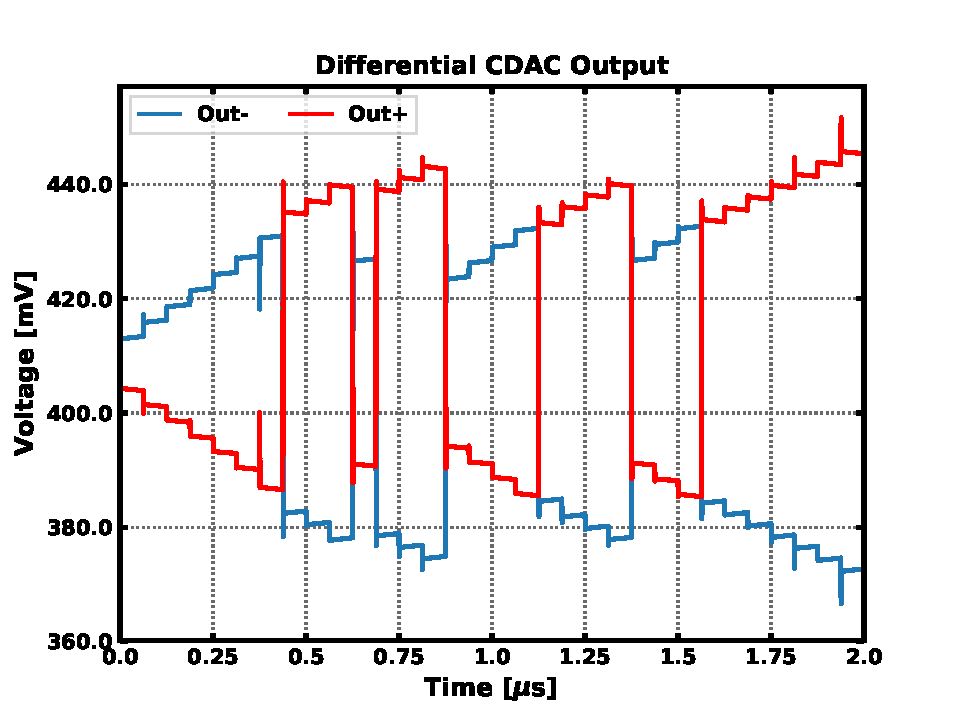
\includegraphics[width=0.65\textwidth, angle=0]{./figs/design/cdac_sw_noise}
		    \caption{Noise spikes in DAC output during switching.}
		    \label{fig:dac_sw_noise}
		\end{figure}
\FloatBarrier
{\color{white}.}
% \normalsize